\documentclass[conference]{IEEEtran}
\IEEEoverridecommandlockouts
\usepackage{cite}
\usepackage{amsmath,amssymb,amsfonts}
\usepackage{algorithmic}
\usepackage{graphicx}
\usepackage{textcomp}
\usepackage{xcolor}
\usepackage{url}
\usepackage{bm}
\usepackage{booktabs}
\usepackage{multirow}

\begin{document}

% =====================================================================
% TITLE AND AUTHOR BLOCK
% >>> REPLACE THE PLACEHOLDER AUTHOR DETAILS BELOW WITH YOUR OWN <<<
% =====================================================================

\title{Parameter-Efficient Adaptation of Frozen Vision--Language Backbones for
Target-Aware Aggression Detection in Bengali Memes}

\author{\IEEEauthorblockN{1\textsuperscript{st} FIRST AUTHOR NAME}
\IEEEauthorblockA{\textit{Department Name} \\
\textit{University Name}\\
City, Country \\
email@example.com}
\and
\IEEEauthorblockN{2\textsuperscript{nd} SECOND AUTHOR NAME}
\IEEEauthorblockA{\textit{Department Name} \\
\textit{University Name}\\
City, Country \\
email@example.com}
}

\maketitle

% =====================================================================
\begin{abstract}
Memes combine an image with embedded text, and this combination is increasingly
used to circulate aggression directed at people on the basis of their politics,
gender or religion. The prevailing response is a purpose-built multimodal
network trained end to end, an approach that is expensive in parameters and, for
low-resource languages such as Bengali, dependent on text encoders and
transcriptions of uneven quality. This work asks whether that expense is
necessary. We adapt a frozen contrastive vision--language backbone using
AdaptFormer, a parallel bottleneck inserted into each residual block, and train
only $1.03\%$ of the network. On MIMOSA, a five-class corpus of 4{,}848 Bengali
memes, this reaches $0.729$ weighted F1 and $0.738$ macro F1 using the image
alone, against $0.718$ and $0.727$ for a faithful reimplementation of the
published multimodal attentive-fusion model that trains $167.4$M parameters and
additionally reads the Bengali caption. We report, as a central finding rather
than a footnote, that a $3{,}841$-parameter linear probe on the same frozen
features already attains $0.695$ weighted F1: roughly two thirds of the margin
over the fusion baseline comes from backbone scale and only one third from the
adapters. A per-block ablation shows adapter utility follows an inverted-U over
depth, and that adapting a single well-chosen block matches adapting all twelve
at one twelfth of the budget. Two further controlled ablations qualify common
assumptions: replacing CLIP with SigLIP inside the fusion model changes weighted
F1 by $0.2\sigma$, and substituting machine OCR for hand-corrected captions on
identical images, splits and labels costs only $0.019$ weighted F1 despite a
median character error rate of $0.788$. Throughout, we estimate run-to-run
variance explicitly and decline to claim differences that fall inside it.
\end{abstract}

\begin{IEEEkeywords}
multimodal classification, parameter-efficient fine-tuning, aggression
detection, low-resource languages, Bengali, vision--language models
\end{IEEEkeywords}

% =====================================================================
\section{Introduction}
\label{sec:intro}
% =====================================================================

Internet memes pair a photograph or illustration with a short piece of text
rendered into the image itself. The format is compact, easily reproduced and
culturally dense, which makes it an efficient vehicle for humour and an equally
efficient vehicle for hostility. Aggressive memes attack individuals or groups,
frequently on the basis of political affiliation, gender or religious identity,
and the attack is often carried by the \emph{interaction} of the two modalities:
an image that is unremarkable on its own acquires an aggressive reading only
when combined with its caption, and vice versa. Detecting such content
automatically is therefore a multimodal problem by construction.

For English, this problem has a mature literature and several benchmark
corpora~\cite{kiela2020,suryawanshi2020,gomez2020}. For Bengali, spoken by more
than 230 million people, the situation is markedly thinner. Annotated
multimodal resources are few~\cite{karim2022,hossain2022b}, and the supporting
infrastructure that English systems take for granted---reliable optical
character recognition, strong pre-trained text encoders, large-scale
image--text pre-training in the target language---is either immature or absent.

The dominant methodological response has been to construct a bespoke multimodal
architecture: encode the image with a pre-trained vision tower, encode the
caption with a language-specific transformer, fuse the two with an attention
mechanism, and train the resulting network end to end. The multimodal attentive
fusion model of Ahsan \emph{et al.}~\cite{ahsan2024}, which defines the corpus
and the task studied here, is a representative and strong instance of this
design. Such models work, but they are expensive: the reimplementation described
in Section~\ref{sec:maf} trains $167.4$ million parameters and produces a
checkpoint of just over one gigabyte.

A parallel development in transfer learning suggests this may be more machinery
than the task requires. Parameter-efficient fine-tuning (PEFT) freezes a large
pre-trained backbone and trains a small number of inserted
parameters~\cite{houlsby2019,hu2021,chen2022}, routinely matching full
fine-tuning at a fraction of the cost. If the visual signal in aggressive memes
is largely carried by a pre-trained vision--language representation, then
adapting that representation cheaply ought to compete with training a
purpose-built fusion network from scratch.

This paper tests that hypothesis and reports the result together with the
controls needed to interpret it honestly. Our contributions are:

\begin{enumerate}
\item \textbf{A parameter-efficient approach that matches multimodal fusion.}
AdaptFormer~\cite{chen2022} applied to a frozen CLIP ViT-L/14 vision tower
reaches $0.729$ weighted F1 while training $1.03\%$ of the parameters and using
only the image, against $0.718$ for a full reimplementation of the published
fusion model that also reads the caption (Section~\ref{sec:results}).

\item \textbf{A control that reattributes that result.} A linear probe on the
same frozen features, with $3{,}841$ trainable parameters, already reaches
$0.695$ weighted F1. Most of the apparent advantage belongs to the backbone, not
to the adapters. We report this prominently because the opposite framing, which
our own first result invited, would have been misleading
(Section~\ref{sec:abl-backbone}).

\item \textbf{A per-block ablation of adapter placement.} Adapter utility over
depth follows an inverted U; the useful capacity sits roughly two thirds of the
way up the tower; and one well-chosen block matches all twelve at one twelfth of
the parameter budget (Section~\ref{sec:abl-block}).

\item \textbf{Two controlled ablations that qualify common assumptions.}
Substituting SigLIP for CLIP inside the fusion architecture changes weighted F1
by $0.2\sigma$ (Section~\ref{sec:abl-encoder}); and replacing hand-corrected
captions with machine OCR on identical images, splits and labels costs $0.019$
weighted F1 despite a median character error rate of $0.788$
(Section~\ref{sec:abl-caption}).

\item \textbf{An explicit noise floor.} We measure seed-to-seed and
run-to-run variance for each training recipe and use it as the threshold for
claiming a difference. Several differences that a single run would have
presented as findings do not survive (Section~\ref{sec:noise}).
\end{enumerate}

Figure~\ref{fig:pipeline} summarises the experimental design: four families of
approach, spanning five orders of magnitude in trainable parameters, evaluated
on one corpus under one protocol.

\begin{figure*}[t]
\centering
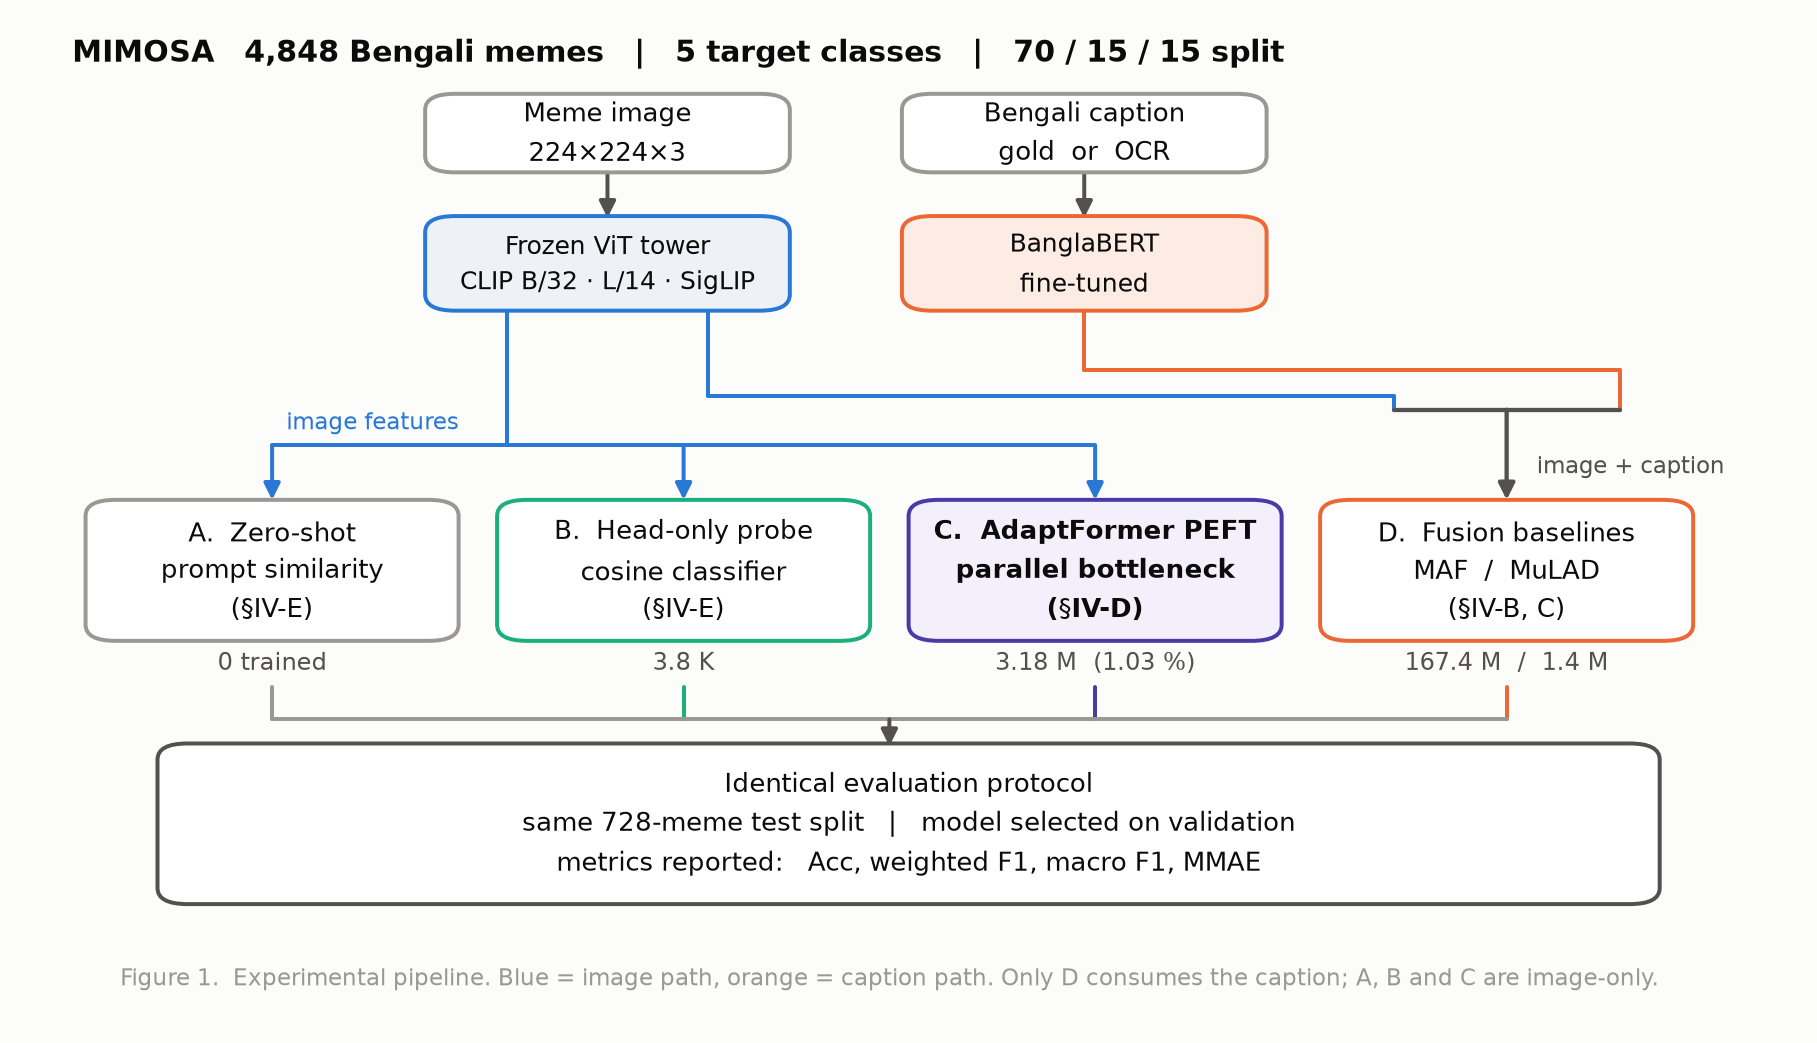
\includegraphics[width=\textwidth]{figures/fig_pipeline.png}
\caption{Experimental pipeline. All four approach families are evaluated on the
same 728-meme test split with the same metrics and the same
selection-on-validation rule. Only the fusion baselines (D) consume the Bengali
caption; A, B and C are image-only.}
\label{fig:pipeline}
\end{figure*}

% =====================================================================
\section{Related Work}
\label{sec:related}
% =====================================================================

\subsection{Unimodal Objectionable Content Detection}

Research on objectionable content detection began, and for a long time remained,
a text-only enterprise. Early work established the task and the difficulty of
annotating it reliably~\cite{ross2017,lekea2018}, and subsequent studies
broadened it across languages through new corpora~\cite{schneider2018,niraula2021}
and new methods~\cite{sreelakshmi2020,sharif2021}. Methodologically, the field
has traced a familiar arc: classical machine learning
approaches~\cite{sreelakshmi2020} gave way to recurrent
architectures~\cite{sharifhoque2021,sadiq2021}, which were in turn superseded by
pre-trained transformer models~\cite{kamal2021,baruah2020,sharif2022}.

Low-resource languages have received growing attention within this line of work.
Sharif and Hoque~\cite{sharif2022} introduced a dataset for identifying
target-aware aggression in Bangla text, establishing the fine-grained
formulation that the present work adopts in a multimodal setting. Comparable
aggression resources have been developed for other under-served
languages~\cite{bhattacharya2020,ranasinghe2021,kumar2023}.

A smaller body of work addresses objectionable content in the visual modality
alone, including the detection of violent or non-compliant
imagery~\cite{gandhi2020}, nudity~\cite{lin2021}, and aggressive or trolling
imagery~\cite{hs2021}. Such approaches are informative but structurally limited
for memes, where the image in isolation is frequently innocuous and the
objectionable meaning arises only in combination with the caption.

\subsection{Multimodal Meme Analysis}

Multimodal resources emerged to address exactly that limitation. Suryawanshi
\emph{et al.}~\cite{suryawanshi2020} released a multimodal dataset for offensive
meme detection, and the Hateful Memes Challenge~\cite{kiela2020} together with
the work of Gomez \emph{et al.}~\cite{gomez2020} established multimodal hate
speech detection as a benchmark problem, notable for being deliberately
constructed so that unimodal models would fail. Pramanick \emph{et
al.}~\cite{pramanick2021a,pramanick2021b} extended the formulation to harmful
memes and, importantly for the present study, to the targets of that harm;
Sharma \emph{et al.}~\cite{sharma2022} pursued the same target-identification
question with named-entity grounding.

Resources for languages other than English followed. Hindi multimodal corpora
have been developed for offensive and hateful meme
identification~\cite{kumari2023,rajput2022}. For Bengali, Karim \emph{et
al.}~\cite{karim2022} and Hossain \emph{et al.}~\cite{hossain2022b} constructed
multimodal hate speech datasets, and related Bengali and Dravidian work has
addressed trolling, offence and sentiment in
memes~\cite{hossain2021,hossain2022c,hasan2022,hossain2022a}. More recent
Bengali work has targeted hateful memes together with their
targets~\cite{hossain2024dora} and the alignment of unimodal features before
fusion~\cite{hossain2024align}.

On the modelling side, early multimodal systems combined modality-specific
representations through comparatively simple fusion
schemes~\cite{hossain2021,hossain2022c,hasan2022}. Attention-based
vision--language architectures subsequently became standard, including
ViLBERT~\cite{lu2019}, contrastively pre-trained models such as
CLIP~\cite{radford2021}, and later alignment-oriented designs such as
ALBEF~\cite{li2021} and BLIP~\cite{li2022}; CLIP representations have been
adapted specifically for hateful meme classification~\cite{kumar2022}, and
zero-shot formulations have been explored for hateful memes with explicit target
modelling~\cite{zhu2022}. Adjacent work on meme sentiment, emotion
and sarcasm~\cite{mishra2023,bandyopadhyay2023} and on analogy-aware offensive
meme detection~\cite{shang2021,zhou2021} further illustrates how much meme
understanding depends on context that neither modality supplies alone. SigLIP~\cite{zhai2023} replaces CLIP's softmax
contrastive objective with a pairwise sigmoid loss and is one of the encoders
compared in Section~\ref{sec:abl-encoder}. A recurring finding across this
literature is that models pre-trained overwhelmingly on English image--text
pairs transfer imperfectly to low-resource languages---a limitation that
Section~\ref{sec:abl-caption} quantifies directly for the text branch.

\subsection{Aggression as a Distinct Construct}

Although multimodal hate and offence detection have advanced considerably,
aggression has been treated less systematically, and multimodal aggression in
low-resource languages least of all. Aggression is not interchangeable with hate
or offence: it denotes a more explicit intent to provoke or harm, and analyses
that collapse these categories lose information that matters both practically
and theoretically~\cite{kocon2021}. Work that does address aggression
multimodally has tended either to treat it as a single undifferentiated
class~\cite{kumari2021,hasan2025mulad} or to focus on a specific target type
such as misogyny~\cite{gasparini2022}. The target-aware formulation adopted
here, in which aggression is decomposed into political, gendered, religious and
other categories alongside a non-aggressive class, retains distinctions that a
binary formulation discards.

\subsection{Parameter-Efficient Transfer Learning}
\label{sec:related-peft}

As pre-trained backbones grew, fully fine-tuning one per downstream task became
impractical, and a family of methods emerged that freeze the backbone and train
a small set of inserted parameters. Houlsby \emph{et al.}~\cite{houlsby2019}
introduced sequential bottleneck adapters for language transformers;
LoRA~\cite{hu2021} instead learns low-rank updates to existing weight matrices
and is now standard for adapting large language models, with a quantised variant
for memory-constrained settings~\cite{dettmers2023}.
AdaptFormer~\cite{chen2022} adapts vision transformers by attaching a
\emph{parallel} bottleneck to the MLP sub-layer of each residual block, which
preserves the frozen computation path exactly and, with a zero-initialised
up-projection, leaves the network numerically unchanged at initialisation. That
last property is unusually convenient for experimental work, because it makes
the untrained model an exact zero-shot baseline measured through the same code
path; Section~\ref{sec:method-peft} makes use of it.

To our knowledge, PEFT has not previously been evaluated for target-aware
multimodal aggression detection in a low-resource language, nor compared against
purpose-built fusion architectures on that task with the parameter budget stated
explicitly.

\subsection{Caption Acquisition and Its Cost}
\label{sec:related-caption}

Multimodal meme models consume an image together with its caption, and published
corpora supply that caption as a column in a distributed data file. For the
corpus used here, those captions were produced by running optical character
recognition over the meme images and then \emph{manually correcting} the output,
precisely because Bengali recognition is unreliable~\cite{ahsan2024,smith2007}.
The reference implementation reads the finished column directly and contains no
extraction stage.

This is a reasonable way to distribute a clean research corpus, but it means the
released artefacts neither include nor evaluate the step that converts a raw
meme image into usable text---a step any deployed system must perform for
itself, and one that manual correction cannot provide at scale. Prior work has
noted the unreliability of Bengali OCR qualitatively; Section~\ref{sec:abl-caption}
measures its cost under a controlled substitution in which images, splits,
labels and hyperparameters are all held fixed and only the caption source
changes.

% =====================================================================
\section{Dataset}
\label{sec:dataset}
% =====================================================================

\subsection{Corpus}

All experiments in Sections~\ref{sec:results}--\ref{sec:error} use
MIMOSA~\cite{ahsan2024}, a corpus of $4{,}848$ Bengali memes annotated for
target-aware aggression. Each instance is an image paired with a Bengali caption
transcribed from that image and a single categorical label; the original
annotation was validated by inter-annotator agreement~\cite{cohen1960}. The corpus is
distributed with a fixed $70/15/15$ partition into $3{,}393$ training, $727$
validation and $728$ test instances, which we use unchanged so that our numbers
remain comparable with the published ones.

\subsection{Class Definitions}

The label set has five values. \textbf{NoAg} (non-aggressive) covers memes with
no aggressive intent. The three targeted aggression classes are \textbf{GAg}
(gendered), \textbf{PAg} (political) and \textbf{RAg} (religious), each denoting
aggression directed at a person or group on that basis. \textbf{Oth} collects
aggression whose target falls outside those three categories---race,
occupation, disability, nationality and so on. Oth is therefore defined
negatively, by what it is not, which turns out to matter considerably for
interpreting the results: it is the hardest class for every model we trained
(Section~\ref{sec:error-confusion}).

Class codes are assigned in the order $\mathrm{NoAg}=0$, $\mathrm{GAg}=1$,
$\mathrm{PAg}=2$, $\mathrm{RAg}=3$, $\mathrm{Oth}=4$, following the original
work so that the ordinal error metric of Section~\ref{sec:metrics} remains
comparable.

\subsection{Distribution}

Table~\ref{tab:dataset} gives the class distribution. The corpus is moderately
imbalanced but far from degenerate: the largest class accounts for $25\%$ of the
training split and the smallest for $17.6\%$. This matters when reading the
baseline comparison in Section~\ref{sec:results-mulad}, because a majority-class
predictor reaches only $0.250$ accuracy here, whereas on strongly skewed
aggression corpora such a predictor can appear deceptively strong.

\begin{table}[t]
\caption{MIMOSA class distribution across the fixed $70/15/15$ partition.}
\label{tab:dataset}
\centering
\small
\begin{tabular}{lrrrr}
\toprule
Class & Train & Validation & Test & Total \\
\midrule
NoAg  & 846 & 181 & 182 & 1{,}209 \\
GAg   & 672 & 144 & 144 & \phantom{0}960 \\
PAg   & 597 & 128 & 128 & \phantom{0}853 \\
RAg   & 618 & 133 & 132 & \phantom{0}883 \\
Oth   & 660 & 141 & 142 & \phantom{0}943 \\
\midrule
Total & 3{,}393 & 727 & 728 & 4{,}848 \\
\bottomrule
\end{tabular}
\end{table}

\subsection{Caption Provenance}
\label{sec:dataset-captions}

The distributed captions are hand-corrected. Measured on the test split, they
average $15.2$ whitespace tokens and $96.6\%$ of their non-space characters are
Bengali script. Section~\ref{sec:abl-caption} constructs a machine-OCR
counterpart over the identical images and compares the two directly; the
statistics of that counterpart are given in Table~\ref{tab:caption-quality}.

% =====================================================================
\section{Method}
\label{sec:method}
% =====================================================================

\subsection{Problem Formulation}
\label{sec:formulation}

Let a meme be a pair $(I, c)$, where $I \in \mathbb{R}^{3 \times 224 \times 224}$
is the resized image and $c$ is its Bengali caption. The task is to predict a
single label $y \in \{0,\dots,K-1\}$ with $K=5$. Every model in this paper
computes a logit vector $\bm{z} \in \mathbb{R}^{K}$ and is trained by minimising
the categorical cross-entropy
\begin{equation}
\mathcal{L} = -\frac{1}{N}\sum_{i=1}^{N} \log \frac{\exp(z_{i,y_i})}{\sum_{k=0}^{K-1}\exp(z_{i,k})} ,
\label{eq:ce}
\end{equation}
where $N$ is the batch size. Cross-entropy treats the five classes as unordered,
which is the correct training objective here even though one of our evaluation
metrics deliberately treats them as ordered
(Section~\ref{sec:metrics}). No class weighting is applied in the main runs; the
imbalance is mild and a weighted variant was tried without measurable benefit.

The approaches differ in which parts of $(I,c)$ they consume and in how many
parameters they update. This is summarised in Table~\ref{tab:approaches} and
elaborated below.

\begin{table}[t]
\caption{The four approach families. ``Trained'' counts parameters receiving
gradients; percentages are of the full network.}
\label{tab:approaches}
\centering
\footnotesize
\begin{tabular}{llrl}
\toprule
Family & Inputs & Trained & Fusion \\
\midrule
Zero-shot (\S\ref{sec:method-controls})     & $I$      & 0                & --- \\
Head-only probe (\S\ref{sec:method-controls}) & $I$    & 3{,}841          & --- \\
AdaptFormer (\S\ref{sec:method-peft})       & $I$      & 3.18\,M (1.03\%) & --- \\
MuLAD (\S\ref{sec:mulad})                   & $I$, $c$ & $\approx$1.4\,M  & concatenation \\
MAF (\S\ref{sec:maf})                       & $I$, $c$ & 167.4\,M         & cross-attention \\
\bottomrule
\end{tabular}
\end{table}

\subsection{Baseline I: Multimodal Attentive Fusion}
\label{sec:maf}

The first baseline is a faithful reimplementation of the multimodal attentive
fusion (MAF) model of Ahsan \emph{et al.}~\cite{ahsan2024}, the architecture
published with this corpus.

\subsubsection{Architecture}
A frozen CLIP ViT-B/32 image encoder~\cite{radford2021} produces a $512$-dimensional
pooled embedding, linearly projected to $768$ and broadcast across the $70$
token positions of the text sequence. A BanglaBERT encoder~\cite{sarker2020},
fine-tuned end to end, produces a $70 \times 768$ contextual sequence for the
caption. A $16$-head attention block fuses them, and the concatenation
$[\,\text{attention output} \mid \text{visual} \mid \text{textual}\,] \in
\mathbb{R}^{70 \times 2304}$ is mean-pooled over the sequence and passed to a
$2304 \rightarrow 128 \rightarrow K$ head.

\subsubsection{A discrepancy in the source material}
The published description states that the query is generated from the textual
features and the key and value from the visual features. The released
implementation does the opposite, computing
$\mathrm{Attn}(Q{=}\text{image},\,K{=}\text{text},\,V{=}\text{image})$. We
default to the released configuration, on the grounds that it is the code that
produced the published numbers, and expose the described configuration as a
switch. Measured on our runs the two differ by $0.007$ weighted F1
($0.718$ versus $0.711$), which is inside the noise floor established in
Section~\ref{sec:noise}; we therefore report them as indistinguishable rather
than ranking them.

\subsubsection{A reproduced defect}
The learning-rate scheduler is constructed for per-optimiser-step advancement
with $\text{epochs} \times |\text{train loader}|$ total steps, but the reference
implementation advances it once per epoch. Over five epochs the learning rate
therefore decays by a negligible fraction and training proceeds at an
effectively constant rate. We reproduce this for fidelity and provide a
corrected variant; correcting it changed weighted F1 by $0.009$
($0.709 \rightarrow 0.718$), again inside the noise floor.

\subsubsection{Optimisation}
AdamW~\cite{loshchilov2019} with learning rate $5\times10^{-5}$, weight decay
$0.01$, batch size $16$, five epochs, maximum caption length $70$. The
checkpoint with the best validation accuracy is retained for testing.

\subsection{Baseline II: Concatenation Fusion}
\label{sec:mulad}

The second baseline is a reimplementation of MuLAD~\cite{hasan2025mulad}, a
simpler and architecturally earlier design from the same research group, which
we include because it isolates the contribution of the fusion mechanism. Its
text branch is one of a CNN, a BiLSTM~\cite{hochreiter1997}, or a CNN followed
by a BiLSTM, over a word-embedding table; its visual branch is a frozen
VGG16~\cite{simonyan2015}, VGG19 or ResNet50~\cite{he2016}; and the two are
joined by plain concatenation followed by a dense classifier. Three embedding
sources are considered: a $64$-dimensional table learned from scratch, and two
$300$-dimensional sets of word vectors trained on the corpus itself.

The full factorial grid is $3 \times 3 \times 3 = 27$ multimodal configurations
plus nine text-only and three image-only baselines, $39$ runs in total. Because
the convolutional towers are frozen, their feature maps are constants; we
precompute and cache them once, which reduces the grid from hours of repeated
convolution to minutes of training dense layers.

Two deviations from the published description are necessary and are recorded
here. The original output layer is a single sigmoid unit trained with binary
cross-entropy, because the corpus it was designed for is binary; we use a
softmax over $K=5$ with Eq.~\eqref{eq:ce}. And the published text reports the
CNN width as $128$ filters in one section and $32$ in another; we adopt $128$,
the value given where the proposed model is described.

\subsection{Proposed: AdaptFormer on a Frozen Backbone}
\label{sec:method-peft}

\subsubsection{The adapted block}
A pre-norm vision transformer block~\cite{dosovitskiy2021} computes
\begin{align}
x &\leftarrow x + \mathrm{Attn}(\mathrm{LN}_1(x)), \label{eq:vit-attn}\\
x &\leftarrow x + \mathrm{MLP}(\mathrm{LN}_2(x)). \label{eq:vit-mlp}
\end{align}
AdaptFormer~\cite{chen2022} leaves Eq.~\eqref{eq:vit-attn} untouched and
replaces Eq.~\eqref{eq:vit-mlp} with
\begin{equation}
x \leftarrow x + \mathrm{MLP}(\mathrm{LN}_2(x))
        + s \cdot W_{\mathrm{up}}\!\left(\mathrm{ReLU}\!\left(W_{\mathrm{down}}(x)\right)\right),
\label{eq:adaptmlp}
\end{equation}
with $W_{\mathrm{down}} \in \mathbb{R}^{r \times d}$,
$W_{\mathrm{up}} \in \mathbb{R}^{d \times r}$, bottleneck $r \ll d$ and a scalar
$s$. The bottleneck branch is \emph{parallel} to the frozen MLP and receives the
same input, so the original computation path is preserved exactly rather than
being displaced. Attention, MLP, layer norms and embeddings all remain frozen;
the adapter budget is $2dr$ parameters per block. Figure~\ref{fig:adaptformer}
contrasts the two blocks.

\begin{figure*}[t]
\centering
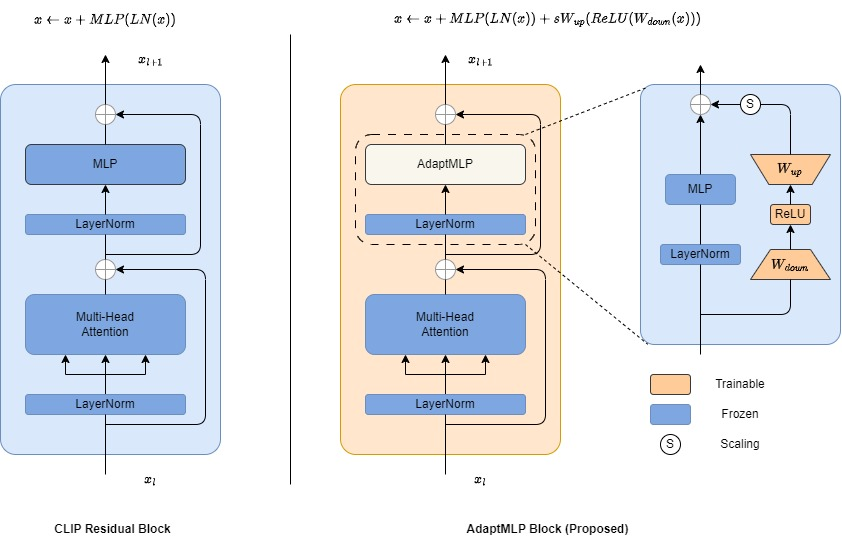
\includegraphics[width=0.95\textwidth]{figures/fig_adaptformer.png}
\caption{The proposed adaptation. AdaptFormer attaches a trainable parallel
bottleneck to the frozen MLP sub-layer of every residual block. Because
$W_{\mathrm{up}}$ is zero-initialised, the adapted network is numerically
identical to the frozen backbone before any gradient step.}
\label{fig:adaptformer}
\end{figure*}

\subsubsection{Zero initialisation and what it buys}
$W_{\mathrm{up}}$ is initialised to zero, so at step $0$ the adapter branch
contributes exactly nothing and the adapted network is bitwise identical to the
frozen backbone---we verified a maximum absolute difference of $0.0$ over a
random batch. Combined with the classifier head described next, this makes the
epoch-$0$ row of the training log a genuine zero-shot measurement taken through
the identical code path, rather than a separately implemented baseline that
might differ for incidental reasons. With mixed precision disabled the two agree
to four decimal places ($36.59\%$ validation accuracy, macro F1 $0.3197$).

\subsubsection{Classifier head}
The head is a cosine classifier whose weights are initialised from CLIP text
embeddings of the class prompts, so that before training the model reproduces
prompt-based zero-shot classification. For $K=5$ classes over a
$d_{\text{feat}}$-dimensional feature this is $K(d_{\text{feat}}+1)$ parameters:
$2{,}561$ for ViT-B/32 and $3{,}841$ for ViT-L/14.

\subsubsection{Design choices}
We follow the reference AdaptFormer configuration: $r=64$, $s=0.1$, parallel
placement, no adapter layer norm, LoRA-style initialisation, adapters in every
block. Section~\ref{sec:abl-block} then asks whether the last of those choices is
justified on this task. Training uses AdamW, learning rate $10^{-3}$, weight
decay $10^{-4}$, batch size $64$ (32 for ViT-L/14), cosine schedule with $10\%$
warmup, gradient clipping at $1.0$, bfloat16 autocast, and ten epochs with the
best-macro-F1 checkpoint on validation retained.

\subsection{Controls}
\label{sec:method-controls}

Two controls make the proposed method interpretable, and we regard them as part
of the method rather than as an afterthought.

\textbf{Zero-shot.} With no training at all, class scores are cosine
similarities between the image embedding and the mean text embedding of a bank
of prompts per class,
\begin{equation}
s(I, k) = \cos\!\big(f_{\text{img}}(I),\; \textstyle\frac{1}{T}\sum_{t=1}^{T} f_{\text{txt}}(p_{t,k})\big).
\label{eq:zeroshot}
\end{equation}
This measures how much of the task is already solved by the pre-trained
representation.

\textbf{Head-only probe.} The same cosine head is trained while every backbone
parameter, adapters included, stays frozen. This isolates the contribution of
the adapters from the contribution of the features they adapt. It is the control
that reframes our headline result in Section~\ref{sec:abl-backbone}, and its
omission is, we suspect, why PEFT results are sometimes over-credited.

% =====================================================================
\section{Experimental Setup}
\label{sec:setup}
% =====================================================================

\subsection{Comparability}

Every number in Sections~\ref{sec:results}--\ref{sec:error} is computed on the
same $728$-meme MIMOSA test split, with the same five classes, the same label
encoding and the same metric implementations. Model selection is performed on
the validation split in every case; the test split is scored once per run and is
never used to choose a configuration, a checkpoint or a hyperparameter. Where a
comparison could not be made under these conditions---the instruction-tuned
vision--language models of Section~\ref{sec:vlm}, which were evaluated on a
different corpus---we report it as a separate setting rather than as an
additional row.

\subsection{Implementation and Hardware}

Models are implemented in PyTorch. The fusion baselines use CLIP via the
reference OpenAI package and BanglaBERT via Hugging Face Transformers; the PEFT
experiments use a standalone AdaptFormer implementation that injects into an
unmodified CLIP vision transformer. Experiments ran on a single GPU with 16\,GB
of memory. Representative training times on this hardware are $13$\,s for a
zero-shot evaluation, $2$\,min $26$\,s for AdaptFormer on ViT-B/32, about
$10$\,min for ViT-L/14, and $5$\,min $18$\,s for MAF.

\subsection{Metrics}
\label{sec:metrics}

We report accuracy, weighted F1, macro F1, and macro-averaged mean absolute
error (MMAE)~\cite{baccianella2009}. Weighted F1 is the primary metric, for
continuity with the published results on this corpus. Macro F1 is reported
alongside it because the classes are unequal and macro F1 refuses to let a large
class conceal failure on a small one---a distinction that matters here, since
Oth is both the smallest concern and the hardest class.

MMAE treats the labels as an ordinal scale and averages the mean absolute error
within each true class:
\begin{equation}
\mathrm{MMAE} = \frac{1}{K}\sum_{k=0}^{K-1} \frac{1}{|S_k|}\sum_{i \in S_k} |\hat{y}_i - y_i| ,
\label{eq:mmae}
\end{equation}
where $S_k$ is the set of test instances whose true label is $k$. The ordering
is inherited from the original work and is a convention rather than a claim
about the semantics of the classes; we report MMAE for comparability and do not
draw conclusions from it alone.

\subsection{Measurement Noise}
\label{sec:noise}

Single runs of these recipes are not reproducible to the precision at which
results are usually reported, and we measured this rather than assuming it.

For the PEFT recipe, four configurations were repeated over three seeds each,
giving a pooled seed-to-seed standard deviation of $0.0067$ macro F1.
Differences below roughly $0.013$ macro F1 are therefore not distinguishable
from noise.

For the MAF recipe the variance is larger. Three seeds of each of two encoder
configurations gave a pooled standard deviation of $0.0159$ weighted F1, so
differences below about $0.03$ weighted F1 are unmeasured. The cause is
structural: five epochs combined with best-checkpoint selection by validation
accuracy on $727$ samples is a high-variance selection rule.

A third measurement is starker still. Two runs of an identical MuLAD
configuration, with the same seed, differed by $0.021$ weighted F1 and agreed on
only $74.7\%$ of their individual test predictions---nondeterminism in GPU
kernel scheduling, not a difference in method.

We use these three figures as thresholds throughout. Where a difference falls
inside the relevant band we say so and decline to rank the configurations, even
when doing so would strengthen the narrative.

% =====================================================================
\section{Results}
\label{sec:results}
% =====================================================================

\subsection{Main Comparison}

Table~\ref{tab:main} reports every approach family on the common test split,
ordered by trainable parameters.

\begin{table*}[t]
\caption{Main results on the MIMOSA test split (728 memes, five classes). ``Trained''
counts parameters receiving gradients. $\dagger$ denotes image-only models.
Differences below $0.03$ weighted F1 within the MAF recipe, and below $0.013$
macro F1 within the PEFT recipe, are inside the noise floor of
Section~\ref{sec:noise}.}
\label{tab:main}
\centering
\small
\begin{tabular}{llrrrrr}
\toprule
Approach & Inputs & Trained & Accuracy & Weighted F1 & Macro F1 & MMAE $\downarrow$ \\
\midrule
Majority class                            & ---            & 0          & 0.250 & 0.080 & 0.080 & --- \\
Zero-shot CLIP ViT-B/32$\dagger$          & image          & 0          & 0.349 & 0.278 & 0.296 & 1.184 \\
Zero-shot CLIP ViT-L/14$\dagger$          & image          & 0          & 0.422 & 0.357 & 0.378 & 1.079 \\
Zero-shot CLIP, caption branch            & caption        & 0          & 0.251 & 0.110 & 0.090 & --- \\
\midrule
Head-only probe, ViT-B/32$\dagger$        & image          & 2{,}561    & 0.628 & 0.630 & 0.639 & --- \\
Head-only probe, ViT-L/14$\dagger$        & image          & 3{,}841    & 0.695 & 0.695 & 0.702 & 0.740 \\
\midrule
MuLAD, best of 39 configurations          & image+caption  & $\approx$1.4\,M & 0.558 & 0.556 & 0.562 & 0.963 \\
AdaptFormer ViT-B/32, $r{=}64$$\dagger$   & image          & 1.19\,M (1.34\%) & 0.644 & 0.645 & 0.653 & 0.835 \\
\textbf{AdaptFormer ViT-L/14, $r{=}64$}$\dagger$ & image    & \textbf{3.18\,M (1.03\%)} & \textbf{0.727} & \textbf{0.729} & \textbf{0.738} & \textbf{0.659} \\
\midrule
MAF (reimplementation)                    & image+caption  & 167.4\,M   & 0.716 & 0.718 & 0.727 & 0.702 \\
MAF, caption source replaced by OCR       & image+caption  & 167.4\,M   & 0.702 & 0.699 & 0.705 & 0.731 \\
MAF with SigLIP encoder, 3 seeds          & image+caption  & $\approx$167\,M & 0.716\,$\pm$\,0.016 & 0.715\,$\pm$\,0.017 & 0.723\,$\pm$\,0.017 & --- \\
MAF with CLIP encoder, 3 seeds            & image+caption  & 167.4\,M   & 0.710\,$\pm$\,0.014 & 0.712\,$\pm$\,0.015 & 0.720\,$\pm$\,0.016 & --- \\
\midrule
\textit{Published MAF}~\cite{ahsan2024}   & image+caption  & 167.4\,M   & \textit{0.741} & \textit{0.742} & --- & \textit{0.645} \\
\bottomrule
\end{tabular}
\end{table*}

\subsection{The Proposed Method Against the Fusion Baseline}

AdaptFormer on ViT-L/14 attains $0.729$ weighted F1 and $0.738$ macro F1,
against $0.718$ and $0.727$ for the MAF reimplementation. The margin,
$+0.011$ weighted F1, is inside the MAF recipe's $0.03$ noise band, so the
correct statement is that \textbf{the two are equal within measurement error}.
That statement is itself the result worth reporting, because the parameter
budgets are not equal: $3.18$\,M against $167.4$\,M, a $53{\times}$ reduction,
with a checkpoint of $12.7$\,MB rather than $1{,}021$\,MB. The proposed method
also never sees the caption.

Performance concentrates exactly where the fusion baseline is weakest.
Table~\ref{tab:perclass} gives per-class F1. On Oth, the negatively defined
catch-all, AdaptFormer ViT-L/14 reaches $0.612$ against MAF's $0.426$---a gain
of $0.186$ on the class that neither zero-shot prompting ($0.226$) nor the
fusion model handles well. On NoAg the gain is smaller but in the same
direction. Conversely MAF retains an advantage on RAg ($0.886$ versus $0.857$),
which is plausibly where the caption carries religious vocabulary that the image
does not show.

\begin{table}[t]
\caption{Per-class F1 on the test split.}
\label{tab:perclass}
\centering
\footnotesize
\begin{tabular}{lrrrrr}
\toprule
Model & NoAg & GAg & PAg & RAg & Oth \\
\midrule
Zero-shot ViT-L/14        & 0.061 & 0.608 & 0.529 & 0.468 & 0.226 \\
Head-only probe ViT-L/14  & 0.644 & 0.661 & 0.800 & 0.836 & 0.568 \\
AdaptFormer ViT-B/32      & 0.586 & 0.614 & 0.776 & 0.779 & 0.511 \\
AdaptFormer ViT-L/14      & 0.654 & 0.712 & \textbf{0.854} & 0.857 & \textbf{0.612} \\
MAF (image + caption)     & 0.626 & 0.633 & 0.807 & \textbf{0.886} & 0.426 \\
MAF + SigLIP              & \textbf{0.675} & \textbf{0.742} & 0.838 & \textbf{0.901} & 0.555 \\
\bottomrule
\end{tabular}
\end{table}

\subsection{Zero-Shot and the Dead Caption Branch}
\label{sec:results-zeroshot}

Zero-shot CLIP is well above chance but roughly half of a trained model:
$0.422$ accuracy at ViT-L/14 against $0.250$ for a majority-class predictor.
Three properties of the failure are informative.

First, \textbf{the caption branch contributes nothing at all}. CLIP's text tower
is English-only, and its byte-pair encoding fragments Bengali into approximately
$135$ near-per-character tokens, so $77\%$ of MIMOSA captions overflow the
$77$-token context window before they are encoded. Caption-only zero-shot scores
$0.251$ accuracy against a $0.250$ majority baseline---exactly nothing. This is
the single clearest illustration in our results of why English-pre-trained
vision--language models transfer poorly to low-resource languages, and it is why
the proposed method treats the image as the only reliable input.

Second, the model \textbf{calls almost everything aggressive}. Collapsed to
binary aggressive/non-aggressive, zero-shot recall is $0.974$ but precision only
$0.751$; it predicts NoAg just $20$ times in $728$. CLIP does detect
hostility-correlated imagery; it has no calibrated notion of an ordinary meme.

Third, \textbf{political and religious targets are visually legible where gender
and Oth are not}. PAg recall reaches $0.805$ and RAg $0.712$---politicians'
faces and religious dress are precisely the content CLIP was pre-trained on---
while Oth scores $0.089$ F1, which is unsurprising for a class defined by
exclusion. The mean pairwise cosine similarity between the five class prompt
embeddings is $0.949$ for ViT-B/32 and $0.898$ for ViT-L/14, so the decision is
being made in a very narrow angular margin.

\subsection{Concatenation Fusion}
\label{sec:results-mulad}

The best of the $39$ MuLAD configurations reaches $0.556$ weighted F1, well
below both the proposed method and MAF. A paired comparison against MAF over the
common test set gives $186$ memes that MAF classifies correctly and MuLAD does
not, against $71$ in the reverse direction; an exact McNemar test~\cite{mcnemar1947}
on the discordant pairs yields $p = 4.7 \times 10^{-13}$. Percentile bootstrap~\cite{efron1979}
intervals over $2{,}000$ resamples do not overlap: $[0.686, 0.750]$ for MAF and
$[0.520, 0.593]$ for MuLAD. This is one of the few differences in the paper
large enough to assert without qualification.

One observation from the grid deserves separate mention because it contradicts
the source publication. MuLAD as published reports that its multimodal fusion
scores \emph{below} its own text-only baseline, and its results table contains a
tuple repeated across roughly eighteen of twenty-seven multimodal
configurations that corresponds exactly to the majority-class share of its test
set---that is, configurations that collapsed to predicting one class for every
input. On MIMOSA we observe neither pathology: no run among our $39$ collapsed,
and fusion improved on both single modalities ($0.556$ against $0.504$ text-only
and $0.509$ image-only). The likely explanation is class balance. The corpus
MuLAD was developed on is split $92/8$ between its two classes, where collapse
is a strong local minimum; MIMOSA's five classes span $17.6\%$ to $25\%$, where
it is not.

% =====================================================================
\section{Ablations}
\label{sec:ablations}
% =====================================================================

\subsection{How Much Is the Adapter, and How Much Is the Backbone?}
\label{sec:abl-backbone}

Our headline comparison invites the reading that AdaptFormer is responsible for
matching MAF. The head-only control shows that reading is wrong, and we consider
this the most important ablation in the paper.

\begin{table}[t]
\caption{Adapters against the frozen features they adapt. The head-only rows
train nothing but the classifier.}
\label{tab:abl-backbone}
\centering
\footnotesize
\begin{tabular}{lrrr}
\toprule
Model & Trained & Weighted F1 & Macro F1 \\
\midrule
ViT-B/32 head-only          & 2{,}561   & 0.630 & 0.639 \\
ViT-B/32 + AdaptFormer      & 1.19\,M   & 0.648 & 0.656 \\
\midrule
ViT-L/14 head-only          & 3{,}841   & 0.695 & 0.702 \\
ViT-L/14 + AdaptFormer      & 3.18\,M   & 0.729 & 0.738 \\
\midrule
MAF (image + caption)       & 167.4\,M  & 0.718 & 0.727 \\
\bottomrule
\end{tabular}
\end{table}

Table~\ref{tab:abl-backbone} shows that a $3{,}841$-parameter linear head on
frozen ViT-L/14 features already reaches $0.695$ weighted F1, which is within
$0.023$ of MAF---inside the MAF noise band. Against that reference, AdaptFormer
adds $0.034$ weighted F1. So of the margin the proposed method holds over the
fusion baseline, \textbf{roughly two thirds is attributable to the backbone
representation and one third to the adapters}.

The adapters' contribution is also scale-dependent. On ViT-B/32 they add $0.017$
macro F1 over head-only, barely outside the $0.013$ noise band; on ViT-L/14 they
add $0.036$, comfortably outside it. The honest summary is that PEFT earns its
place on the larger tower and is close to unnecessary on the smaller one, and
that anyone reporting a PEFT result on this task without a head-only control
will overstate what the method contributes.

\subsection{Which Blocks Earn an Adapter?}
\label{sec:abl-block}

The reference configuration adapts every block. We tested whether that is
justified by training one model per block with adapters attached to that block
alone, on ViT-B/32 ($12$ blocks, $r=64$, ten epochs), with repeated seeds on
four configurations to establish the noise band.

\begin{table}[t]
\caption{Per-block adapter ablation, ViT-B/32. Seed-to-seed standard deviation
over the four repeated configurations is $0.0067$; differences below
$\sim$$0.013$ macro F1 are noise.}
\label{tab:abl-block}
\centering
\footnotesize
\begin{tabular}{lrrr}
\toprule
Adapted & Trained & Macro F1 & Seeds \\
\midrule
Block 0  & 101{,}697 & 0.6325\,$\pm$\,0.0077 & 3 \\
Block 3  & 101{,}697 & 0.6552 & 1 \\
Block 5  & 101{,}697 & 0.6579 & 1 \\
\textbf{Block 7} & 101{,}697 & \textbf{0.6655} & 1 \\
Block 8  & 101{,}697 & 0.6596\,$\pm$\,0.0104 & 3 \\
Block 9  & 101{,}697 & 0.6614 & 1 \\
Block 11 & 101{,}697 & 0.6326 & 1 \\
\midrule
Head only (floor)      & 2{,}561     & 0.6389\,$\pm$\,0.0057 & 3 \\
All 12 blocks (ceiling)& 1{,}192{,}193 & 0.6559\,$\pm$\,0.0032 & 3 \\
\bottomrule
\end{tabular}
\end{table}

Three findings follow from Table~\ref{tab:abl-block}.

\textbf{Adapter utility follows an inverted U over depth.} Blocks $7$--$9$ are
best ($0.660$--$0.666$); the first and last blocks are worst ($0.633$). The
spread of $0.033$ across depth is about $2.5\times$ the noise band, so the shape
is real even though adjacent blocks are not separable from one another. The
interpretation is mechanical: early blocks encode generic edges and textures
that need no task adaptation, and the final block sits too close to the output
to reshape anything downstream. Useful capacity is roughly two thirds of the way
up.

\textbf{One well-chosen block matches all twelve.} Block $7$ at $0.6655$ against
all-blocks at $0.6559 \pm 0.0032$ is a $+0.0096$ gap that falls inside the noise
band, so they tie---at one twelfth of the adapter budget ($101$\,K against
$1.19$\,M). Adapting every block, the reference setting, buys nothing
measurable on this task.

\textbf{Adapting the earliest block is no better than adapting nothing.} Block
$0$ scores $0.6325 \pm 0.0077$ against a head-only floor of
$0.6389 \pm 0.0057$: within about one standard deviation, so it gives nothing
rather than actively hurting.

We note one methodological point. A single-seed run initially showed block $8$
beating all-blocks by $+0.017$, which would have been a publishable-looking
result; over three seeds its mean is $0.6596 \pm 0.0104$ and the effect
disappears. This is precisely the class of claim the noise band exists to catch.

\subsection{Does the Vision Encoder Matter?}
\label{sec:abl-encoder}

We replaced CLIP ViT-B/32 with SigLIP base/16~\cite{zhai2023} inside the MAF
architecture, holding everything else fixed---the same attention operands, the
same head, the same optimiser and schedule, the same selection rule. Running
both encoders through one pipeline is what makes the comparison meaningful; we
confirmed the CLIP arm reproduces the reference parameter counts exactly
($255{,}297{,}797$ total, $167{,}448{,}581$ trainable).

Over three seeds each, SigLIP reaches $0.7151 \pm 0.0173$ weighted F1 and CLIP
$0.7117 \pm 0.0145$. The difference of $+0.0034$ against a pooled standard
deviation of $0.0159$ is $0.2\sigma$: \textbf{the two encoders are
indistinguishable on this task}. Per-seed values overlap almost completely.
SigLIP is about $35\%$ faster per epoch ($41$\,s against $64$\,s), which is a
real if undramatic reason to prefer it.

Two secondary findings are worth recording. \emph{Preprocessing must travel with
the encoder.} Feeding SigLIP the ImageNet normalisation constants costs $0.030$
weighted F1, while doing the same to CLIP costs nothing measurable---CLIP's
channel means $[0.481, 0.458, 0.408]$ are almost exactly ImageNet's, whereas
SigLIP expects $[0.5,0.5,0.5]$ with standard deviation $[0.5,0.5,0.5]$. A
normalisation mismatch that is harmless for one encoder is a genuine defect for
another. \emph{Richer visual tokens do not help this fusion.} Supplying SigLIP's
$196$ patch tokens instead of a single pooled vector scores $0.7070$ against
$0.7151$, no gain, because MAF uses the image as both query and value and then
mean-pools the fused sequence---richer tokens are averaged back down. Exploiting
a patch sequence would require redesigning the fusion, not merely feeding it
more.

\subsection{Modality and Fusion}
\label{sec:abl-modality}

The MuLAD grid provides a clean modality ablation, since the same fusion head is
trained over text-only, image-only and concatenated inputs. Best weighted F1 was
$0.504$ text-only, $0.509$ image-only and $0.556$ fused: concatenation fusion
recovers about $0.05$ over either modality alone. Read together with
Section~\ref{sec:results-zeroshot}, where CLIP's Bengali caption branch
contributes nothing, and with the proposed method, which ignores the caption
entirely and still matches MAF, the picture is consistent. The caption carries
real signal, but only when read by an encoder that actually models Bengali, and
even then it adds less than the choice of vision backbone.

\begin{figure}[t]
\centering
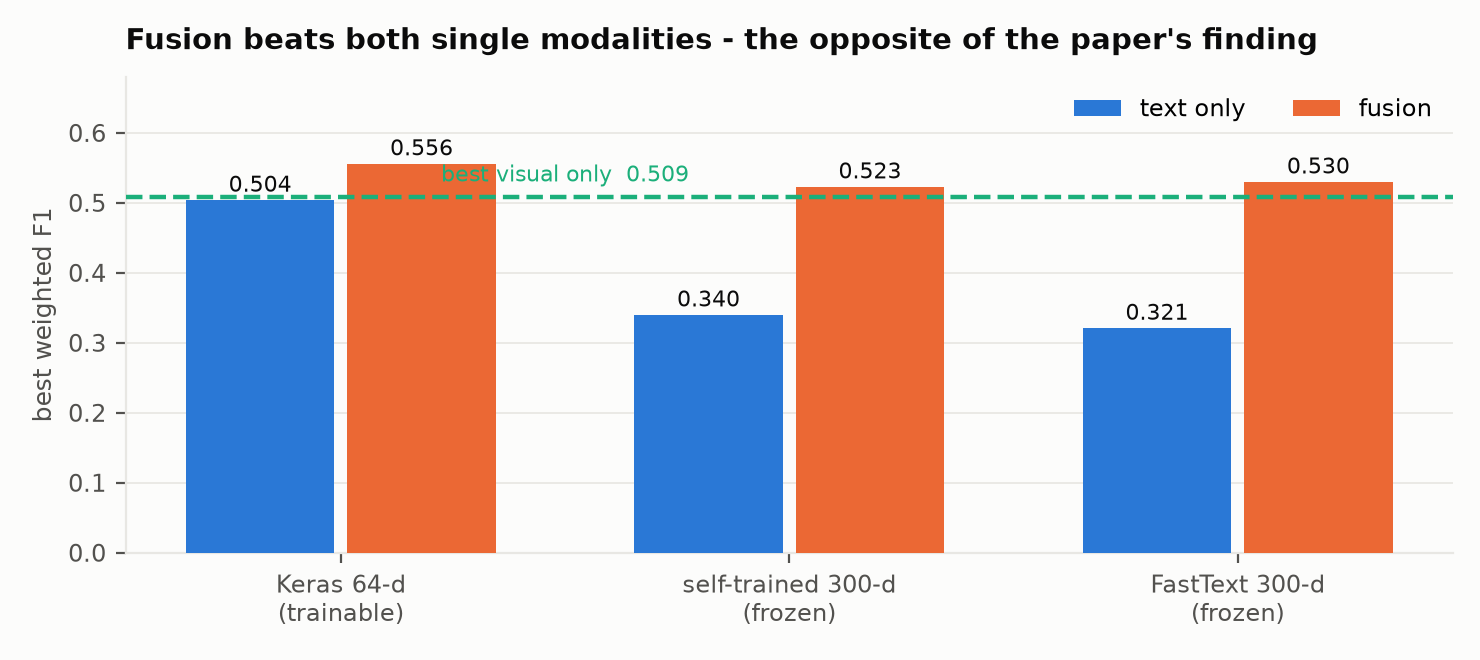
\includegraphics[width=\columnwidth]{figures/fig_modality.png}
\caption{Modality ablation over the MuLAD grid. Concatenation fusion improves on
both single modalities, in contrast to the pathology reported for this
architecture on a strongly imbalanced binary corpus.}
\label{fig:modality}
\end{figure}

Figure~\ref{fig:modality} shows the effect across all three embedding sources.
One limitation of our grid must be stated. The two $300$-dimensional embedding
variants were held frozen while the $64$-dimensional table was trained end to
end, so their much weaker results ($0.239$ and $0.340$ weighted F1 text-only,
against $0.504$) confound embedding source with trainability. We therefore do
not claim that pre-trained embeddings are worse here, only that frozen
corpus-trained $300$-dimensional vectors underperformed a trainable
$64$-dimensional table.

\subsection{What Does Caption Quality Actually Cost?}
\label{sec:abl-caption}

Section~\ref{sec:related-caption} argued that corpora distribute hand-corrected
captions and thereby conceal a stage every deployed system must perform. We
measured its cost directly.

Tesseract's LSTM engine~\cite{smith2007} with Bengali script support was run
over all $4{,}848$ MIMOSA images, using sparse-text page segmentation selected
on evidence rather than left at the default. The resulting captions replaced the
distributed ones in the split files while \emph{image, label, split membership,
architecture, hyperparameters and seed were all held fixed}. Caption source is
the only variable.

\begin{table}[t]
\caption{Machine OCR against the distributed hand-corrected captions, measured
over the same 4{,}848 images. CER and WER are normalised by gold length and are
uncapped, so values above $1.0$ indicate more inserted error than original text.}
\label{tab:caption-quality}
\centering
\footnotesize
\begin{tabular}{lrr}
\toprule
Measure & Hand-corrected & Machine OCR \\
\midrule
Bengali character share      & 0.966 & 0.462 \\
Latin character share        & 0.000 & 0.453 \\
Tokens with no Bengali       & 0.029 & 0.527 \\
Mean caption length (tokens) & 15.2  & 28.9 \\
\midrule
Median character error rate  & ---   & 0.788 \\
Mean character error rate    & ---   & 1.061 \\
Mean word error rate         & ---   & 2.245 \\
Memes with CER $>0.5$        & ---   & 75.8\% \\
\bottomrule
\end{tabular}
\end{table}

Table~\ref{tab:caption-quality} shows the OCR output is severely degraded. The
median character error rate is $0.788$; $75.8\%$ of memes exceed $0.5$; more
than half of all OCR tokens contain no Bengali character at all; and the output
is $1.96\times$ longer than the gold text, the excess being watermarks, channel
branding and spurious Latin fragments. A representative failure has the
recogniser capturing a publisher's watermark and truncating the actual meme
text.

\begin{figure}[t]
\centering
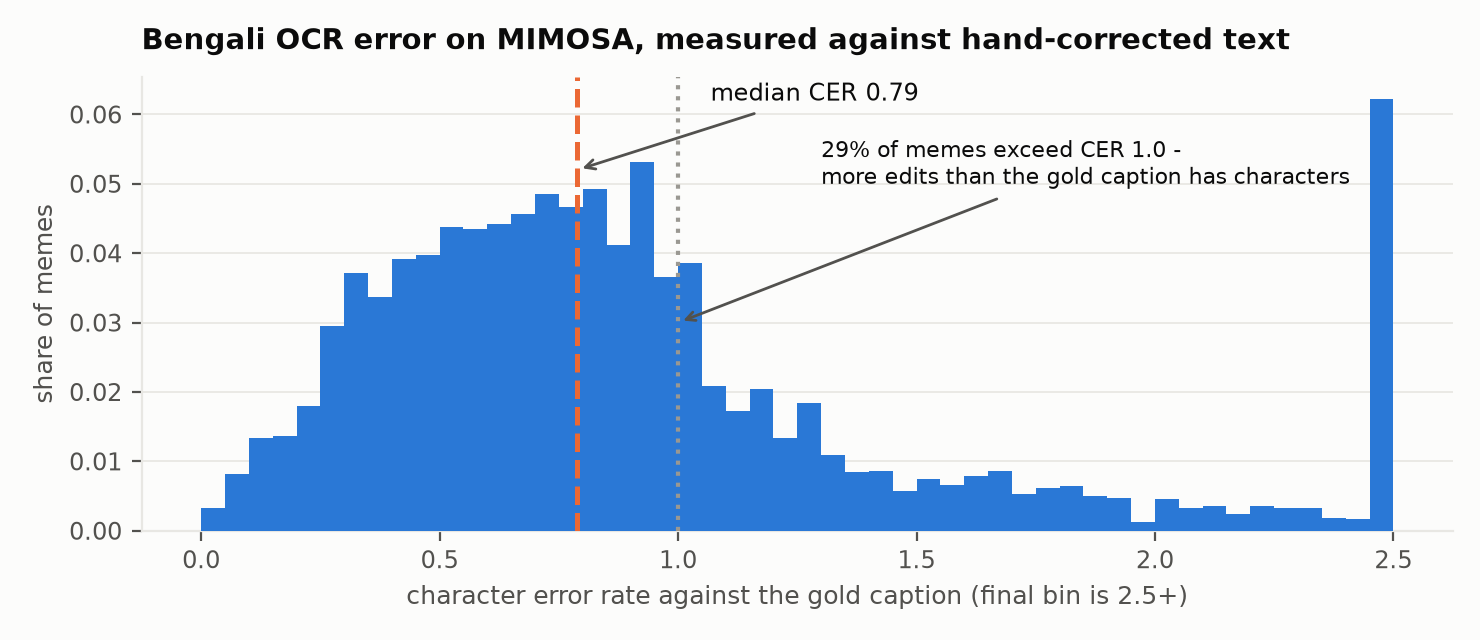
\includegraphics[width=\columnwidth]{figures/fig_cer.png}
\caption{Distribution of character error rate for machine OCR against the
hand-corrected captions, over all 4{,}848 MIMOSA memes. The rate is normalised
by gold length and uncapped, so the mass beyond $1.0$ is memes for which the
recogniser inserted more error than there was original text.}
\label{fig:cer}
\end{figure}

Figure~\ref{fig:cer} gives the full distribution.
The effect on the model is much smaller than that damage suggests.
\textbf{Weighted F1 falls from $0.718$ to $0.699$, a loss of $0.019$}---itself
inside the MAF recipe's noise band. Two conclusions follow, and the second is
the one we did not expect.

First, the result is good news for deployment: an end-to-end Bengali meme
classifier that must perform its own transcription loses very little relative to
one handed clean text, even with a transcription pipeline this poor.

Second, and more informatively, \textbf{MAF is far less dependent on its caption
than its architecture implies}. A model whose text branch genuinely drove its
predictions could not absorb a median $0.788$ character error rate for $0.019$
weighted F1. This corroborates, from the opposite direction, the finding of
Section~\ref{sec:abl-backbone}: the discriminative signal on this corpus sits
predominantly in the visual representation. We note that an uncontrolled
comparison---the same architecture trained on a different, smaller, four-class
OCR'd corpus---would have suggested a loss of $0.154$ weighted F1, eight times
larger. That comparison would have been wrong, and it is a useful illustration
of why the matched-pair design matters.

% =====================================================================
\section{Error Analysis}
\label{sec:error}
% =====================================================================

\subsection{Confusion Structure}
\label{sec:error-confusion}

Errors are not distributed uniformly across classes. For MAF, per-class recall
runs from $0.92$ on RAg down to $0.63$ on Oth, and the dominant off-diagonal
mass is NoAg and GAg being absorbed into Oth ($18\%$ of NoAg instances). Oth is
the sink for uncertainty in every model we trained, which follows from its
definition: it is the residual category, so it has no positive visual or lexical
signature for a model to learn. The clearest practical implication of this work
for corpus design is that a negatively defined class will bound the achievable
macro F1 regardless of architecture.

\begin{figure}[t]
\centering
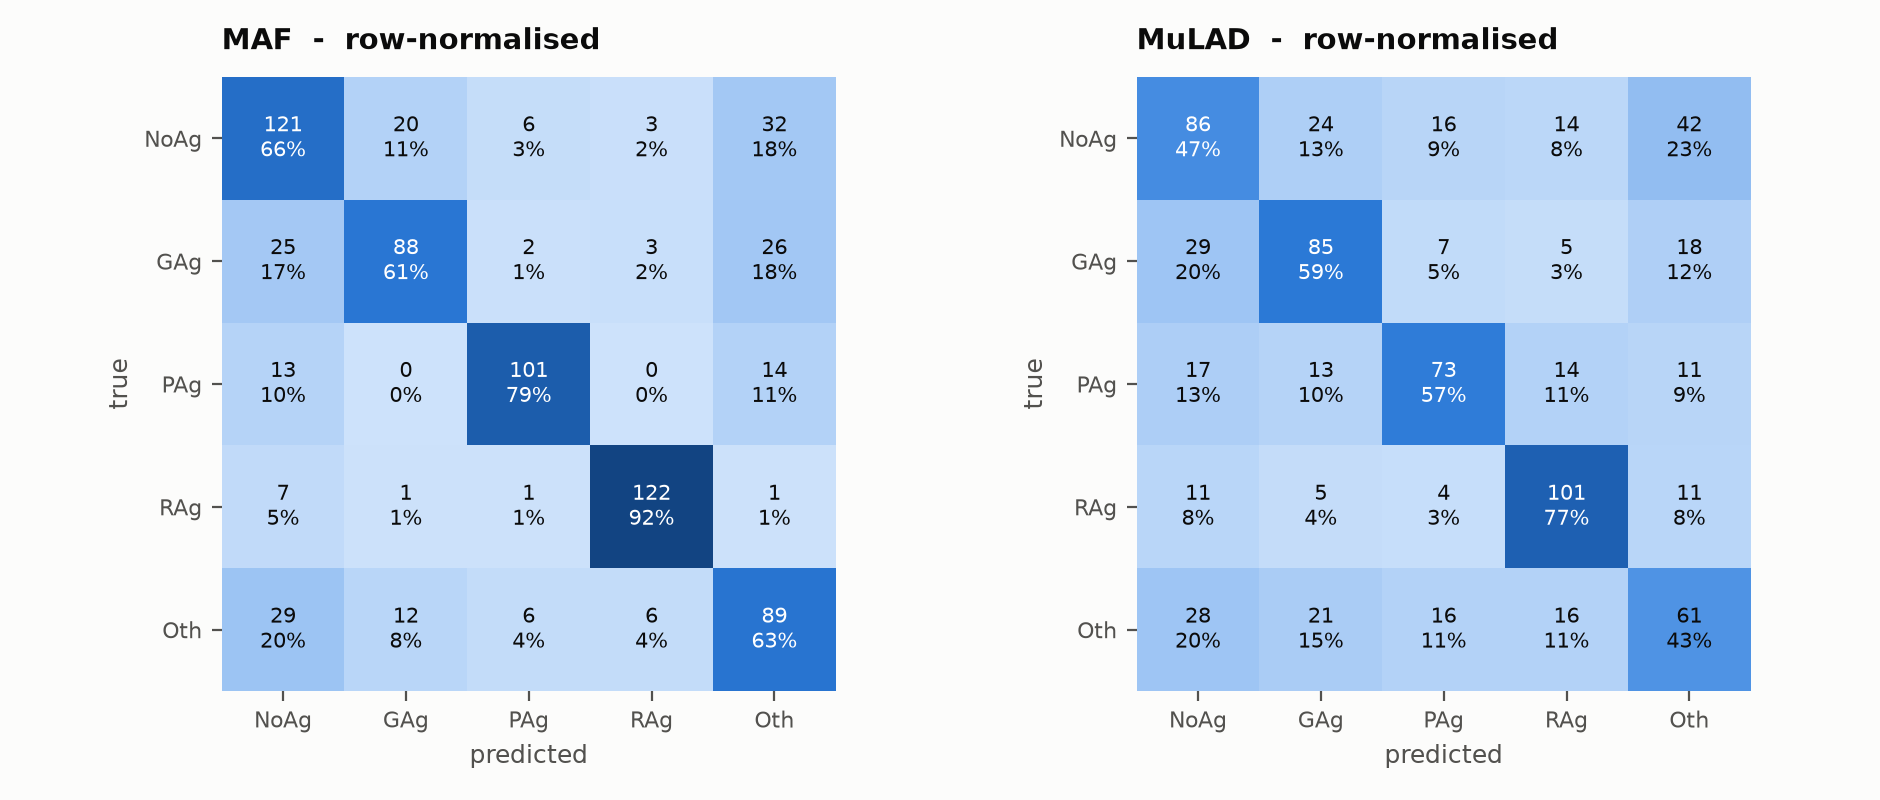
\includegraphics[width=\columnwidth]{figures/fig_confusion.png}
\caption{Row-normalised confusion matrices for the cross-attention fusion
baseline (left) and the best concatenation-fusion configuration (right). Oth
absorbs misclassified NoAg and GAg instances in both.}
\label{fig:confusion}
\end{figure}

Figure~\ref{fig:confusion} shows the structure for both fusion baselines.
Partitioning the test set by which models succeed sharpens the point. Of $728$
memes, $335$ are classified correctly by both MAF and the best MuLAD
configuration, $186$ by MAF alone, $71$ by MuLAD alone, and $136$ by neither.
Within that jointly misclassified set the concentration is uneven---$24\%$ of
NoAg and $24\%$ of Oth instances, against only $6\%$ of RAg---so the residual
difficulty is a property of the ambiguous classes rather than of the models.

\subsection{Error Severity}

Because the label ordering is ordinal by convention, the magnitude of an error
is informative as well as its frequency. MAF attains MMAE $0.702$ against
MuLAD's $0.963$, so MAF's mistakes are not merely fewer but land nearer the true
class. AdaptFormer ViT-L/14 improves further to $0.659$.

\subsection{Calibration}

Confidence and correctness are poorly aligned for the concatenation baseline.
MuLAD's mean maximum softmax probability on the test split is $0.815$ against an
accuracy of $0.558$: it is systematically overconfident by roughly $26$ points,
and its reliability curve lies below the diagonal in every confidence bin. Any
deployment that used a confidence threshold to route items for human review
would be badly misled. Figure~\ref{fig:reliability} plots the reliability curve. We did not investigate temperature scaling, which is the
obvious remedy.

% =====================================================================
\section{A Second Setting: Instruction-Tuned Vision--Language Models}
\label{sec:vlm}
% =====================================================================

An adjacent question is whether a large general-purpose vision--language model
solves this task without task-specific training at all. We evaluated
Qwen3-VL-8B-Instruct~\cite{qwen3vl} in two regimes: prompted zero-shot
classification, and QLoRA~\cite{dettmers2023} supervised fine-tuning with rank
$16$ on the attention projections.

These experiments were run on a different corpus---a four-class, $400$-meme
test split with machine-OCR captions---and are therefore \textbf{not comparable}
with Table~\ref{tab:main}. We report them as a self-contained setting with its
own baseline, and we explicitly do not rank them against the MIMOSA results.

\begin{table}[t]
\caption{Second setting: four-class corpus, 400-meme test split, machine-OCR
captions. Internally consistent; not comparable with Table~\ref{tab:main}.}
\label{tab:vlm}
\centering
\footnotesize
\begin{tabular}{llrr}
\toprule
Model & Regime & Accuracy & Weighted F1 \\
\midrule
MAF                 & trained on this corpus & 0.460 & 0.451 \\
Qwen3-VL-8B         & QLoRA fine-tuned       & 0.680 & 0.682 \\
\textbf{Qwen3-VL-8B} & \textbf{zero-shot}    & \textbf{0.720} & \textbf{0.716} \\
\bottomrule
\end{tabular}
\end{table}

Two results in Table~\ref{tab:vlm} are striking. The instruction-tuned model,
with no exposure to the training corpus, outperforms the task-specific model
trained on it by $0.265$ weighted F1. And fine-tuning that model on the corpus
made it \emph{worse}, by $0.034$. With roughly $2{,}400$ training instances,
low-rank supervised adaptation appears to degrade a strong general prior rather
than sharpen it---a failure mode consistent with the broader observation in this
paper that, on this task, most of the usable signal already resides in
large-scale pre-training.

% =====================================================================
\section{Limitations}
\label{sec:limitations}
% =====================================================================

Several constraints bound what we can claim.

\textbf{Single-corpus scope.} All comparable results are on MIMOSA. The finding
that the visual modality dominates may be a property of this corpus---whose
political and religious targets are unusually visually legible---rather than of
Bengali aggressive memes generally.

\textbf{Seeds.} The noise bands of Section~\ref{sec:noise} rest on three seeds
per configuration, which is enough to disqualify small differences but not to
place tight intervals on large ones. Ten of the twelve per-block configurations
in Table~\ref{tab:abl-block} are single-seed and inherit that uncertainty.

\textbf{An unresolved pipeline discrepancy.} The CLIP arm of our unified
encoder-comparison pipeline scores $0.7117 \pm 0.0145$ weighted F1, while the
original reference implementation scores $0.667$ under nominally identical
architecture and hyperparameters, verified by parameter count and near-identical
loss curves. The two differ in checkpoint selection epoch, in floating-point
precision of the loaded CLIP weights, and in which random number generators are
seeded. We could not close this gap and therefore compare only within a single
pipeline; readers should not compare our SigLIP numbers against the $0.667$
figure.

\textbf{A confounded embedding ablation.} As stated in
Section~\ref{sec:abl-modality}, the pre-trained embedding variants were frozen
while the learned table was not.

\textbf{Prompt sensitivity.} The zero-shot and head-only results depend on a
prompt bank we did not tune extensively; the mean inter-class prompt similarity
of $0.898$--$0.949$ suggests substantial headroom remains.

\textbf{Explanation.} We report where and how models fail but not why at the
level of individual features. Attribution over the visual branch, and
cross-attention inspection for MAF, are the natural next step.

% =====================================================================
\section{Conclusion}
\label{sec:conclusion}
% =====================================================================

We set out to test whether target-aware aggression detection in Bengali memes
requires a purpose-built multimodal network trained end to end. It does not. A
frozen CLIP ViT-L/14 adapted with AdaptFormer reaches $0.729$ weighted F1 while
training $1.03\%$ of its parameters and reading only the image, statistically
indistinguishable from a faithful reimplementation of the published fusion model
that trains $167.4$M parameters and additionally consumes the Bengali caption.

The more useful contribution may be the controls. A $3{,}841$-parameter probe on
the same frozen features reaches $0.695$, so most of the advantage belongs to
backbone scale rather than to parameter-efficient fine-tuning. One adapted block
out of twelve matches all twelve. Swapping CLIP for SigLIP moves the result by
$0.2\sigma$. And replacing hand-corrected captions with machine OCR whose median
character error rate is $0.788$ costs only $0.019$ weighted F1---strong
converging evidence that the discriminative signal on this corpus is
predominantly visual, and that the caption branch of a multimodal aggression
detector may be doing considerably less work than its architecture diagram
suggests.

Two directions follow naturally. The first is to pair an adapted vision tower
with a text encoder that genuinely models Bengali, rather than with CLIP's
English-only tower, which our zero-shot analysis shows cannot read the caption
at all. The second is to address the Oth class at the level of annotation rather
than architecture: a category defined by exclusion places a ceiling on macro F1
that no amount of modelling has removed.

\begin{figure}[t]
\centering
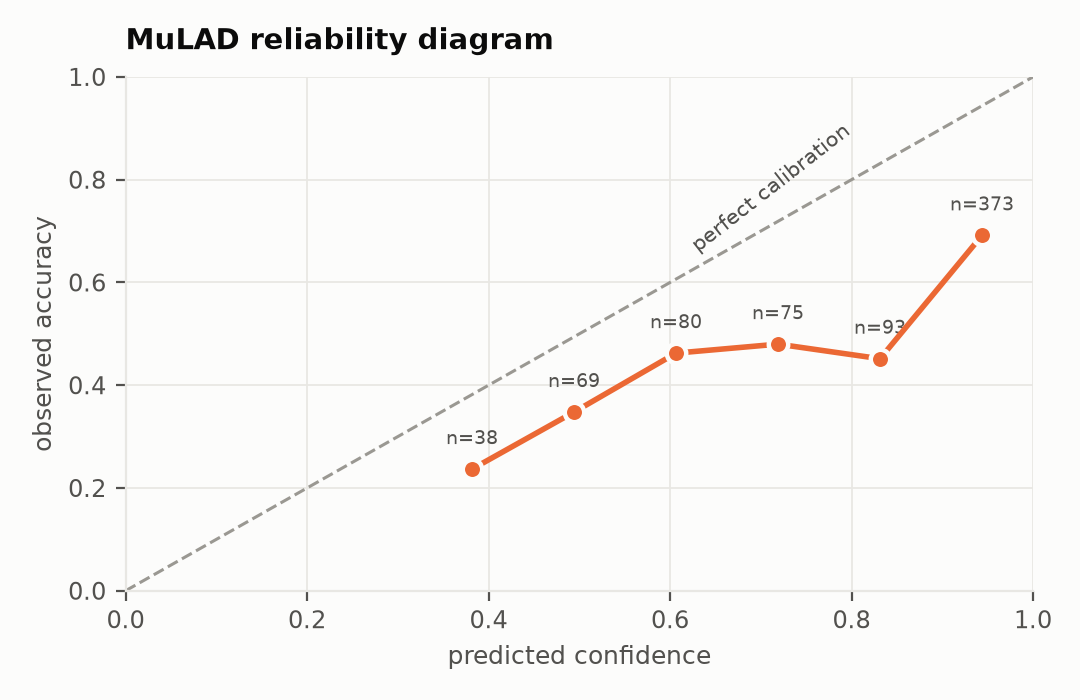
\includegraphics[width=0.85\columnwidth]{figures/fig_reliability.png}
\caption{Reliability diagram for the concatenation-fusion baseline. The curve
lies below the diagonal in every bin: the model is systematically overconfident.}
\label{fig:reliability}
\end{figure}

% =====================================================================
\begin{thebibliography}{00}

\bibitem{suryawanshi2020} S. Suryawanshi, B. R. Chakravarthi, M. Arcan, and P. Buitelaar, ``Multimodal meme dataset (MultiOFF) for identifying offensive content in image and text,'' in \textit{Proc. 2nd Workshop on Trolling, Aggression and Cyberbullying}, 2020, pp. 32--41.

\bibitem{kiela2020} D. Kiela \textit{et al.}, ``The hateful memes challenge: Detecting hate speech in multimodal memes,'' in \textit{Advances in Neural Information Processing Systems}, vol. 33, 2020, pp. 2611--2624.

\bibitem{pramanick2021b} S. Pramanick \textit{et al.}, ``MOMENTA: A multimodal framework for detecting harmful memes and their targets,'' 2021, arXiv:2109.05184.

\bibitem{kocon2021} J. Koco\'{n} \textit{et al.}, ``Offensive, aggressive, and hate speech analysis: From data-centric to human-centered approach,'' \textit{Information Processing \& Management}, vol. 58, no. 5, p. 102643, 2021.

\bibitem{kumari2021} K. Kumari, J. P. Singh, Y. K. Dwivedi, and N. P. Rana, ``Multi-modal aggression identification using convolutional neural network and binary particle swarm optimization,'' \textit{Future Generation Computer Systems}, vol. 118, pp. 187--197, 2021.

\bibitem{sharif2022} O. Sharif and M. M. Hoque, ``Tackling cyber-aggression: Identification and fine-grained categorization of aggressive texts on social media using weighted ensemble of transformers,'' \textit{Neurocomputing}, vol. 490, pp. 462--481, 2022.

\bibitem{karim2022} M. R. Karim, S. K. Dey, T. Islam, M. Shajalal, and B. R. Chakravarthi, ``Multimodal hate speech detection from Bengali memes and texts,'' in \textit{Proc. Int. Conf. on Speech and Language Technologies for Low-resource Languages}, 2022, pp. 293--308.

\bibitem{hossain2022b} E. Hossain, O. Sharif, and M. M. Hoque, ``MUTE: A multimodal dataset for detecting hateful memes,'' in \textit{Proc. 2nd Conf. of the Asia-Pacific Chapter of the ACL and 12th Int. Joint Conf. on Natural Language Processing: Student Research Workshop}, 2022, pp. 32--39.

\bibitem{ahsan2024} S. Ahsan, E. Hossain, O. Sharif, A. Das, M. M. Hoque, and M. A. A. Dewan, ``A multimodal framework to detect target aware aggression in memes,'' in \textit{Proc. 18th Conf. of the European Chapter of the ACL (Volume 1: Long Papers)}, 2024, pp. 2487--2500.

\bibitem{smith2007} R. Smith, ``An overview of the Tesseract OCR engine,'' in \textit{Proc. 9th Int. Conf. on Document Analysis and Recognition (ICDAR)}, 2007, pp. 629--633.

\bibitem{ross2017} B. Ross \textit{et al.}, ``Measuring the reliability of hate speech annotations: The case of the European refugee crisis,'' 2017, arXiv:1701.08118.

\bibitem{lekea2018} I. K. Lekea and P. Karampelas, ``Detecting hate speech within the terrorist argument: A Greek case,'' in \textit{Proc. IEEE/ACM Int. Conf. on Advances in Social Networks Analysis and Mining (ASONAM)}, 2018, pp. 1084--1091.

\bibitem{schneider2018} J. M. Schneider, R. Roller, P. Bourgonje, S. Hegele, and G. Rehm, ``Towards the automatic classification of offensive language and related phenomena in German tweets,'' in \textit{Proc. 14th Conf. on Natural Language Processing (KONVENS)}, 2018, p. 95.

\bibitem{niraula2021} N. B. Niraula, S. Dulal, and D. Koirala, ``Offensive language detection in Nepali social media,'' in \textit{Proc. 5th Workshop on Online Abuse and Harms (WOAH)}, 2021, pp. 67--75.

\bibitem{sreelakshmi2020} K. Sreelakshmi, B. Premjith, and K. P. Soman, ``Detection of hate speech text in Hindi-English code-mixed data,'' \textit{Procedia Computer Science}, vol. 171, pp. 737--744, 2020.

\bibitem{sharif2021} O. Sharif, E. Hossain, and M. M. Hoque, ``NLP-CUET@DravidianLangTech-EACL2021: Offensive language detection from multilingual code-mixed text using transformers,'' in \textit{Proc. 1st Workshop on Speech and Language Technologies for Dravidian Languages}, 2021, pp. 255--261.

\bibitem{sharifhoque2021} O. Sharif and M. M. Hoque, ``Identification and classification of textual aggression in social media: Resource creation and evaluation,'' in \textit{Proc. Int. Workshop on Combating Online Hostile Posts in Regional Languages during Emergency Situation}, 2021, pp. 9--20.

\bibitem{sadiq2021} S. Sadiq \textit{et al.}, ``Aggression detection through deep neural model on Twitter,'' \textit{Future Generation Computer Systems}, vol. 114, pp. 120--129, 2021.

\bibitem{kamal2021} O. Kamal, A. Kumar, and T. Vaidhya, ``Hostility detection in Hindi leveraging pre-trained language models,'' in \textit{Combating Online Hostile Posts in Regional Languages during Emergency Situation}. Cham, Switzerland: Springer, 2021, pp. 213--223.

\bibitem{baruah2020} A. Baruah, K. Das, F. Barbhuiya, and K. Dey, ``Aggression identification in English, Hindi and Bangla text using BERT, RoBERTa and SVM,'' in \textit{Proc. 2nd Workshop on Trolling, Aggression and Cyberbullying}, Marseille, France, 2020, pp. 76--82.

\bibitem{bhattacharya2020} S. Bhattacharya \textit{et al.}, ``Developing a multilingual annotated corpus of misogyny and aggression,'' 2020, arXiv:2003.07428.

\bibitem{ranasinghe2021} T. Ranasinghe and M. Zampieri, ``Multilingual offensive language identification for low-resource languages,'' \textit{Transactions on Asian and Low-Resource Language Information Processing}, vol. 21, no. 1, pp. 1--13, 2021.

\bibitem{gandhi2020} S. Gandhi \textit{et al.}, ``Scalable detection of offensive and non-compliant content/logo in product images,'' in \textit{Proc. IEEE/CVF Winter Conf. on Applications of Computer Vision (WACV)}, 2020, pp. 2247--2256.

\bibitem{lin2021} X. Lin, F. Qin, Y. Peng, and Y. Shao, ``Fine-grained pornographic image recognition with multiple feature fusion transfer learning,'' \textit{International Journal of Machine Learning and Cybernetics}, vol. 12, pp. 73--86, 2021.

\bibitem{hs2021} C. Hs \textit{et al.}, ``TrollMeta@DravidianLangTech-EACL2021: Meme classification using deep learning,'' in \textit{Proc. 1st Workshop on Speech and Language Technologies for Dravidian Languages}, 2021, pp. 277--280.

\bibitem{gomez2020} R. Gomez, J. Gibert, L. Gomez, and D. Karatzas, ``Exploring hate speech detection in multimodal publications,'' in \textit{Proc. IEEE/CVF Winter Conf. on Applications of Computer Vision (WACV)}, 2020, pp. 1470--1478.

\bibitem{pramanick2021a} S. Pramanick \textit{et al.}, ``Detecting harmful memes and their targets,'' 2021, arXiv:2110.00413.

\bibitem{kumari2023} G. Kumari, D. Bandyopadhyay, and A. Ekbal, ``EmoffMeme: Identifying offensive memes by leveraging underlying emotions,'' \textit{Multimedia Tools and Applications}, pp. 1--36, 2023.

\bibitem{rajput2022} K. Rajput, R. Kapoor, K. Rai, and P. Kaur, ``Hate me not: Detecting hate inducing memes in code switched languages,'' 2022, arXiv:2204.11356.

\bibitem{hossain2021} E. Hossain, O. Sharif, and M. M. Hoque, ``NLP-CUET@DravidianLangTech-EACL2021: Investigating visual and textual features to identify trolls from multimodal social media memes,'' in \textit{Proc. 1st Workshop on Speech and Language Technologies for Dravidian Languages}, 2021, pp. 300--306.

\bibitem{hossain2022c} E. Hossain \textit{et al.}, ``Identification of multilingual offense and troll from social media memes using weighted ensemble of multimodal features,'' \textit{Journal of King Saud University - Computer and Information Sciences}, vol. 34, no. 9, pp. 6605--6623, 2022.

\bibitem{hasan2022} M. Hasan, N. Jannat, E. Hossain, O. Sharif, and M. M. Hoque, ``CUET-NLP@DravidianLangTech-ACL2022: Investigating deep learning techniques to detect multimodal troll memes,'' in \textit{Proc. 2nd Workshop on Speech and Language Technologies for Dravidian Languages}, 2022, pp. 170--176.

\bibitem{hossain2022a} E. Hossain, O. Sharif, and M. M. Hoque, ``MemoSen: A multimodal dataset for sentiment analysis of memes,'' in \textit{Proc. 13th Language Resources and Evaluation Conf. (LREC)}, 2022, pp. 1542--1554.

\bibitem{lu2019} J. Lu, D. Batra, D. Parikh, and S. Lee, ``ViLBERT: Pretraining task-agnostic visiolinguistic representations for vision-and-language tasks,'' in \textit{Advances in Neural Information Processing Systems}, vol. 32, 2019.

\bibitem{radford2021} A. Radford \textit{et al.}, ``Learning transferable visual models from natural language supervision,'' in \textit{Proc. Int. Conf. on Machine Learning (ICML)}, 2021, pp. 8748--8763.

\bibitem{li2021} J. Li \textit{et al.}, ``Align before fuse: Vision and language representation learning with momentum distillation,'' in \textit{Advances in Neural Information Processing Systems}, vol. 34, 2021, pp. 9694--9705.

\bibitem{li2022} J. Li, D. Li, C. Xiong, and S. Hoi, ``BLIP: Bootstrapping language-image pre-training for unified vision-language understanding and generation,'' in \textit{Proc. Int. Conf. on Machine Learning (ICML)}, 2022, pp. 12888--12900.

\bibitem{kumar2022} G. K. Kumar and K. Nanadakumar, ``Hate-CLIPper: Multimodal hateful meme classification based on cross-modal interaction of CLIP features,'' 2022, arXiv:2210.05916.

\bibitem{mishra2023} S. Mishra \textit{et al.}, ``Memotion 3: Dataset on sentiment and emotion analysis of codemixed Hindi-English memes,'' 2023, arXiv:2303.09892.

\bibitem{bandyopadhyay2023} D. Bandyopadhyay \textit{et al.}, ``A knowledge infusion based multitasking system for sarcasm detection in meme,'' in \textit{Proc. European Conf. on Information Retrieval (ECIR)}, 2023, pp. 101--117.

\bibitem{shang2021} L. Shang \textit{et al.}, ``AOMD: An analogy-aware approach to offensive meme detection on social media,'' \textit{Information Processing \& Management}, vol. 58, no. 5, p. 102664, 2021.

\bibitem{zhou2021} Y. Zhou, Z. Chen, and H. Yang, ``Multimodal learning for hateful memes detection,'' in \textit{Proc. IEEE Int. Conf. on Multimedia \& Expo Workshops (ICMEW)}, 2021, pp. 1--6.

\bibitem{gasparini2022} F. Gasparini, G. Rizzi, A. Saibene, and E. Fersini, ``Benchmark dataset of memes with text transcriptions for automatic detection of multi-modal misogynistic content,'' \textit{Data in Brief}, vol. 44, p. 108526, 2022.

\bibitem{cohen1960} J. Cohen, ``A coefficient of agreement for nominal scales,'' \textit{Educational and Psychological Measurement}, vol. 20, no. 1, pp. 37--46, 1960.
\bibitem{houlsby2019} N. Houlsby \textit{et al.}, ``Parameter-efficient transfer learning for NLP,'' in \textit{Proc. Int. Conf. on Machine Learning (ICML)}, 2019, pp. 2790--2799.

\bibitem{hu2021} E. J. Hu \textit{et al.}, ``LoRA: Low-rank adaptation of large language models,'' 2021, arXiv:2106.09685.

\bibitem{chen2022} S. Chen \textit{et al.}, ``AdaptFormer: Adapting vision transformers for scalable visual recognition,'' in \textit{Advances in Neural Information Processing Systems}, vol. 35, 2022, pp. 16664--16678.

\bibitem{dettmers2023} T. Dettmers, A. Pagnoni, A. Holtzman, and L. Zettlemoyer, ``QLoRA: Efficient finetuning of quantized LLMs,'' in \textit{Advances in Neural Information Processing Systems}, vol. 36, 2023, pp. 10088--10115.

\bibitem{zhai2023} X. Zhai, B. Mustafa, A. Kolesnikov, and L. Beyer, ``Sigmoid loss for language image pre-training,'' in \textit{Proc. IEEE/CVF Int. Conf. on Computer Vision (ICCV)}, 2023, pp. 11975--11986.

\bibitem{dosovitskiy2021} A. Dosovitskiy \textit{et al.}, ``An image is worth 16x16 words: Transformers for image recognition at scale,'' in \textit{Proc. Int. Conf. on Learning Representations (ICLR)}, 2021.

\bibitem{sarker2020} S. Sarker, ``BanglaBERT: Bengali mask language model for Bengali language understanding,'' 2020. [Online]. Available: \url{https://github.com/sagorbrur/bangla-bert}

\bibitem{loshchilov2019} I. Loshchilov and F. Hutter, ``Decoupled weight decay regularization,'' in \textit{Proc. Int. Conf. on Learning Representations (ICLR)}, 2019.

\bibitem{hochreiter1997} S. Hochreiter and J. Schmidhuber, ``Long short-term memory,'' \textit{Neural Computation}, vol. 9, no. 8, pp. 1735--1780, 1997.

\bibitem{simonyan2015} K. Simonyan and A. Zisserman, ``Very deep convolutional networks for large-scale image recognition,'' in \textit{Proc. Int. Conf. on Learning Representations (ICLR)}, 2015.

\bibitem{he2016} K. He, X. Zhang, S. Ren, and J. Sun, ``Deep residual learning for image recognition,'' in \textit{Proc. IEEE Conf. on Computer Vision and Pattern Recognition (CVPR)}, 2016, pp. 770--778.

\bibitem{baccianella2009} S. Baccianella, A. Esuli, and F. Sebastiani, ``Evaluation measures for ordinal regression,'' in \textit{Proc. 9th Int. Conf. on Intelligent Systems Design and Applications}, 2009, pp. 283--287.

\bibitem{mcnemar1947} Q. McNemar, ``Note on the sampling error of the difference between correlated proportions or percentages,'' \textit{Psychometrika}, vol. 12, no. 2, pp. 153--157, 1947.

\bibitem{efron1979} B. Efron, ``Bootstrap methods: Another look at the jackknife,'' \textit{The Annals of Statistics}, vol. 7, no. 1, pp. 1--26, 1979.

\bibitem{qwen3vl} Qwen Team, ``Qwen3-VL: A versatile vision-language model family,'' 2025. [Online]. Available: \url{https://github.com/QwenLM/Qwen3-VL}

\bibitem{hasan2025mulad} M. M. Hasan, S. Ahsan, M. M. Hoque, and M. A. A. Dewan, ``MuLAD: Multimodal aggression detection from social media memes exploiting visual and textual features,'' in \textit{Proc. Int. Conf. on Pattern Recognition and Artificial Intelligence}, 2025.

\bibitem{sharma2022} S. Sharma, M. S. Akhtar, P. Nakov, and T. Chakraborty, ``DISARM: Detecting the victims targeted by harmful memes,'' in \textit{Findings of the Association for Computational Linguistics: NAACL}, 2022, pp. 1572--1588.

\bibitem{zhu2022} J. Zhu, R. K.-W. Lee, and W. H. Chong, ``Multimodal zero-shot hateful meme detection,'' in \textit{Proc. 14th ACM Web Science Conf.}, 2022, pp. 382--389.

\bibitem{kumar2023} R. Kumar \textit{et al.}, ``A multilingual, multimodal dataset of aggression and bias: The ComMA dataset,'' \textit{Language Resources and Evaluation}, pp. 1--81, 2023.

\bibitem{hossain2024align} E. Hossain, O. Sharif, M. M. Hoque, and S. M. Preum, ``Align before attend: Aligning visual and textual features for multimodal hateful content detection,'' 2024, arXiv:2402.09738.

\bibitem{hossain2024dora} E. Hossain, O. Sharif, M. M. Hoque, and S. M. Preum, ``Deciphering hate: Identifying hateful memes and their targets,'' 2024, arXiv:2403.10829.

\end{thebibliography}

\end{document}
